\documentclass[beamer]{standalone}%

\begin{document}

\begin{frame}\frametitle{Що таке АММ?}
  \begin{block}{Автоматизовані Маркет Мейкери}
    АММ (або автоматизовані маркет мейкери) --- це механізм автоматизованого
    трейдингу електроними валютами, що визначений математичними формулами,
    законами, правилами.
  \end{block}

  \begin{figure}
    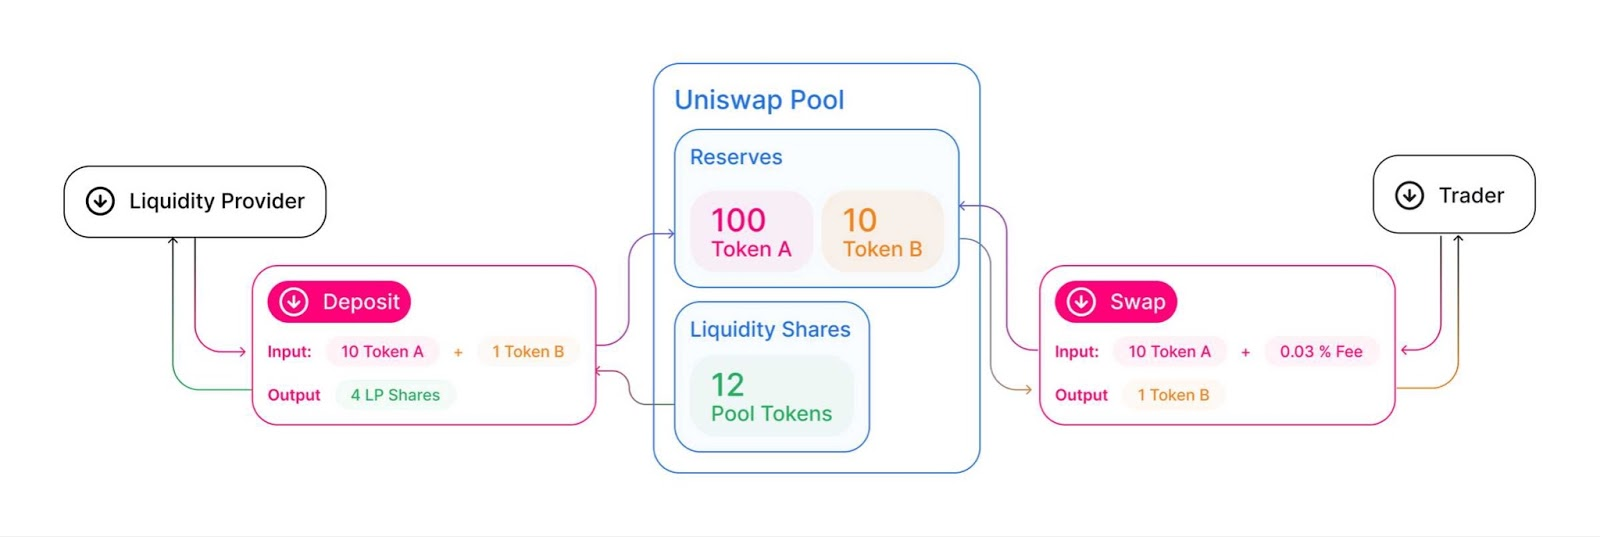
\includegraphics[scale=0.2]{./presentation/images/amm-intro-example.jpeg}
  \end{figure}
\end{frame}

\end{document}
